\documentclass[../Bachelorarbeit.tex]{subfiles}
\begin{document}

\graphicspath{{./figures/theory/nw/}}	%specifying the folder for the figures

\section{Complex Networks}
\label{sec:theory_complexNetworks}
This thesis lays its main focus on the influence of network-topologies on the equilibrium found in continuous double-auction. The networks define the neighbourhood between agents and determine which pair of agents can trade with each other. All graph-related definitions in the following sections are provided through \cite{Drmota2007}.

\medskip

A network is a graph \textit{G = (V,E)} which has a finite set of vertices \textit{V = V(G)} and a finite set of edges \textit{E = E(G)}. The vertices resemble the agents and the edges connecting them resemble the neighbourhood between agents or the knowledge of each other. Two agents know each other and can trade with each other if there exists an edge between them. In this context only undirected graphs consisting of undirected edges $e$ $\in$ $E(G)$, $e = {v_1, v_2}$ between two vertices $v_1$, $v_2$ $\in$ $V(G)$ without multi- and self-edges are of interest.

\begin{itemize}
\item Undirected: if one agent $v_1$ knows another agent $v_2$ then $v_2$ knows $v_1$ too - trading is always possible in both directions.
\item No multi-edges: one neighbourhood connection is enough as edges have no additional properties or weights.
\item No self-edges: agents are not allowed to trade with themselves.
\end{itemize}

This thesis also investigates the equilibrium in so called \textit{complex networks} which are a special kind of networks which exhibit small-world properties and follow a power-law distribution which are discussed shown below. In the following sections a short overview of the development of network-topologies and recent findings in this research-field is given and the complex networks used in this thesis are discussed. See appendix \ref{app:topologies} for a complete catalogue of network-topologies investigated in this thesis - the complex ones are:

\begin{enumerate}
\item Erdos-Renyi
\item Barbasi-Albert
\item Watts-Strogatz
\end{enumerate}

M.E.J. Newmann gives an extensive overview of complex networks in the paper \cite{Newman_ComplexNetworks} which in combination of the books \cite{Jackson2008} and \cite{Easley2010} are the main sources for the following sections. Note that in this thesis only static networks are of interest thus no models of network-growth or processes in and on networks are discussed.

\subsection{Overview}
Since the first proof in network-theory by Euler in 1735 the analysis of networks has had a long tradition. In recent years the focus is shifting away from the analysis of single small graphs and the properties of individual vertices or edges to consideration of large-scale statistical properties of graphs TODO: das ist kopiert, umformulieren. This transition of focus was made possible by the availability of an ever increasing amount of processing power through computers which allow the investigation of networks with millions of vertices.

\subsection{Random graphs}
One of the simplest network models studied was the random graph which was investigated first by \cite{ErdosRenyi_RandomGraphs}. Such networks are constructed by having n unconnected vertices and then adding at random each possible edge with a given probability. The probabilities can follow different distributions e.g. a uniform- poisson- or gaussian-distribution. The Ascending-Connected topology with random short-cuts is a random graph constructed using the uniform-distribution - see appendix \ref{app:topologies}. 

TODO: noch in paper newman und buch jackson nachlesen

\subsection{Small-World effects}
In 1960s Stanley Milgram conducted a famous experiment in which he demonstrated that a letter can reach a destination person by an average of just 6 intermediate steps in between. In his work \cite{TraverMilgram_StudySmallWorld} \citep{Milgram_SmallWorld} he termed this phenomenon the \textit{small-world effect}. Although the results of his work have been questioned - more specifically that the world is really a small one e.g. by \cite{Kleinfeld_BigWorld} - it had big influences within the network-research community and led to the development of the small-world property. It is of very importance e.g. in social networks because this property implies that information spreads very quickly in the network as it needs very few steps to reach all nodes. This can also be applied to trading networks where it enables traders to trade goods within very few intermediary steps to traders which value the good the most.

\medskip

To calculate whether a network has the small-world property one starts with the formula given by \cite{Newman_ComplexNetworks} for calculating the average path length in a network

\begin{center}
$\ell = \frac{1}{\frac{1}{2}n(n+1)} \displaystyle\sum_{i \geq j }^{} d_{ij}$
\end{center}

where $d_{ij}$ is the shortest distance from vertex i to vertex j. Networks then exhibit the small-world property if $\ell$ scales at max logarithmically with network size of mean degree.

\subsection{Scale-free networks}
Researchers found that real-world networks are non-random which lead to the discovery of the phenomena of scale-free networks which are networks whose vertex-degree distribution follows a power-law.

\subsubsection{Degree distribution}
In an undirected Graph \textit{G} the edges adjacent to $v$ $\in$ $V(G)$ 

\begin{center}
$\Gamma(v)$ = ${w \in V(G) | vw \in E(G)}$
\end{center}

are the neighbours. The quantity of the neighbours of $v$ $\in$ $V(G)$ 

\begin{center}
$d(v) = |\Gamma(v)|$ = $|{w \in V(G) | vw \in E(G)}|$
\end{center}

is the degree of a vertex $v$ $\in$ $V(G)$. When regarding the adjacent-matrix of a graph the degree of a vertex $v_i$ $\in$ $V(G)$ is given by

\begin{center}
$d(v_i) = \displaystyle\sum_{j=1}^{n} a_{ij}$
\end{center}

Having defined the degree of a vertex one can calculate the degree distribution of of a given network simply by counting the number of nodes which have a given degree k:

\begin{center}
$P_{deg}(k) = fraction of nodes in the graph with degree k$
\end{center}

The resulting statistics is presented in a histogram which gives a good visual overview of the distribution of the degrees and allows to calculate the average degree. 

TODO: show histogram and average degree of a random-network.

\subsubsection{Power-law distribution}
In the figure TODO: ref the degree-distribution of a few examples of real-world networks are shown.

TODO: show histogram of a scale-free network. from thesis

What is striking about this figure is the long right tail which follows a power-law 

\begin{center}
$P_{deg}(k) \sim k^{-\gamma}$
\end{center}

Note that due to the power-law the distribution of such scale-free networks remains unchanged when scaling \textit{k} with a given factor \textit{a}. Thus those networks are called \textit{scale-free}.

\begin{figure}[H]
	\centering
  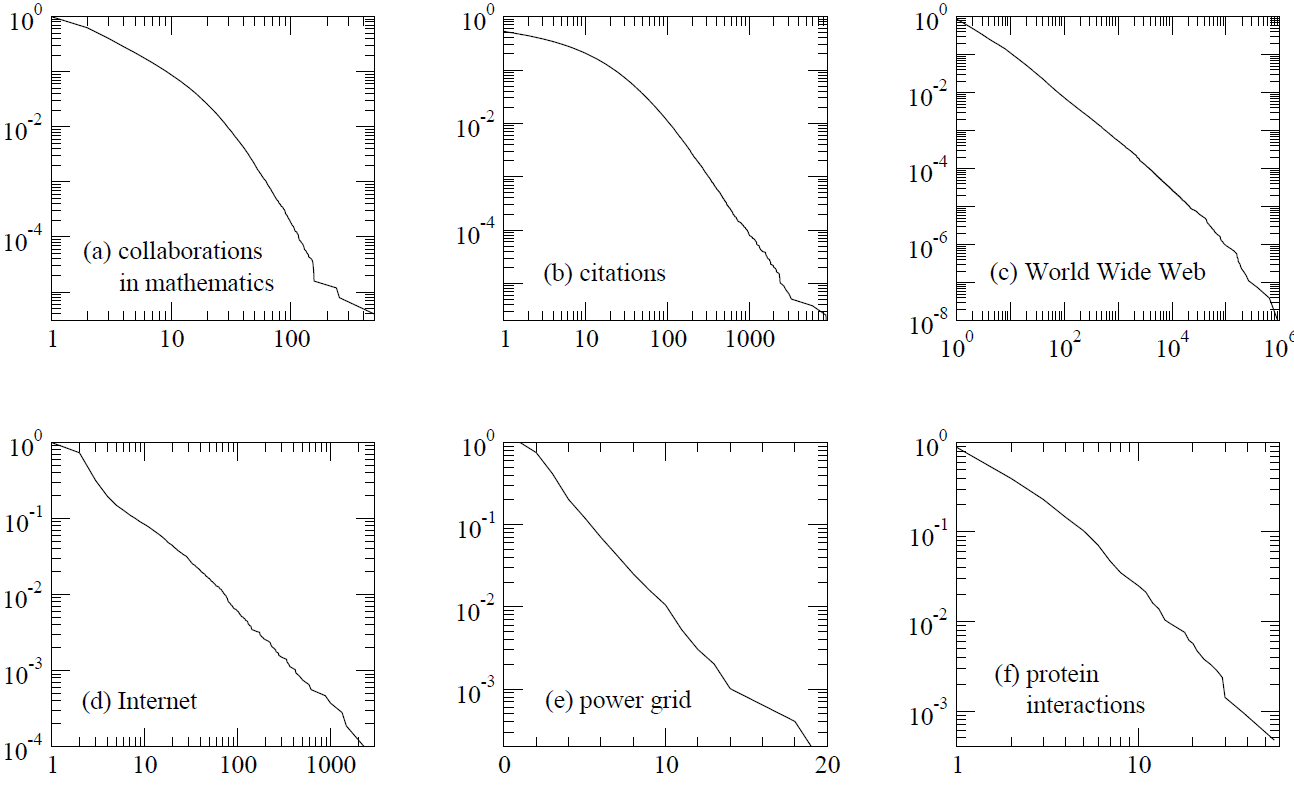
\includegraphics[width=1.0\textwidth, angle=0]{SCALEFREE_REALWORLD_EXAMPLES.png}
  	\caption{Examples for degree-distributions of real-world networks. Diagram taken from \cite{Newman_ComplexNetworks} }
	\label{fig:SCALEFREE_REALWORLD_EXAMPLES}
\end{figure}

Note that a straight line in a log-lop plot is evidence of a power-law distribution thus only (c), (d) and (f) appear to have power-law distributions.

\medskip
The strengths of scale-free networks is their resilience against \textit{random} removal of vertices.

\begin{figure}[H]
	\centering
  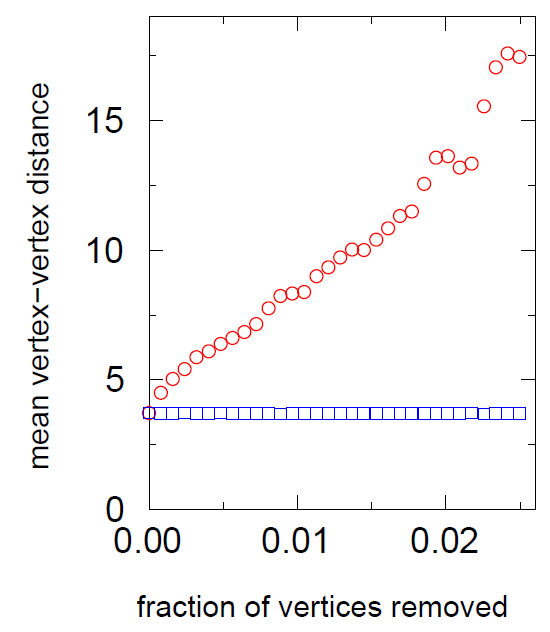
\includegraphics[width=0.5\textwidth, angle=0]{RESILIENCE.png}
  	\caption{Random removal of vertices increases the average path length very slightly. Removing vertices with highest degree first increases the average path length rapidly. Diagram taken from \cite{Newman_ComplexNetworks} }
	\label{fig:RESILIENCE}
\end{figure}

This can be applied to scale-free trading networks too where the ausfall of a random trader won't impair the overall trading ability but if an important hub fails then the overall trading performance could be affected. TODO: genauer ausformulieren. ausfall eines traders in dieser thesis: kein goods oder kein cash mehr bzw. kann nichtmehr traden.

\subsection{Complex Network examples}
Complex Networks: are Small-World and/or Scale-Free \citep{BarratWeigt_PropertiesSmallWorld} \citep{AmaralScalaStanley_ClassesSmallWorld}
Such networks are termed \textit{scale-free} networks \cite{BarabasiAlbert_EmergenceScaling}
Small World and Scale Free Network:  A scale free network as defined by Barabasi and Albert \citep{BarabasiAlbert_EmergenceScaling}, is a network where the degree distribution follows a power law.

In this section the complex networks used in this thesis as outlined above are described and how they \textit{in general} can be generated. All of them exhibit small-world properties and follow a power-law distribution. TODO: wirklich beides?

\subsubsection{Erdos-Renyi}
random-graph

\subsubsection{Barbasi-Albert}
\cite{BarabasiAlbert_EmergenceScaling}

\subsubsection{Watts-Strogatz}
\cite{WattsStrogatz_DynamicsSmallWorld}

start with a small regular lattice and add shortcuts.
then rewire edges to create small-world properties
the rewireing process allows the small-world model to interpolate between a regular latice and something 

\end{document}